\documentclass[12pt]{article}

\usepackage[spanish]{babel}
\usepackage{hyperref}
\usepackage{graphicx}
\usepackage{listings}
\usepackage{color}
\usepackage{multicol}
\usepackage{amssymb}
\spanishdecimal{.}
\usepackage{enumitem}
\usepackage{here}
\usepackage{dsfont}
\usepackage{amsmath}


%% Título
\title{Matemáticas para las Ciencias Aplicadas I}
\title{
	Segunda Lista de Problemas \\
	\textbf{Primera Parte} \\
	\vspace{1ex}
	\large Matemáticas para las Ciencias Aplicadas I \\
	Facultad de Ciencias, UNAM}

%% Fecha
\date{\today}

%% Autor
\author{Flores Morán Julieta Melina \\ Zarco Romero José Antonio}

%% Se marca el inicio del documento.
\begin{document}

%% Comando para crear el título.
\maketitle

%1
\section{Ejercicio 3}
\begin{enumerate}[label=(\alph*)]
\item Aproximar el valor del límite
\[
\lim_{x \to 0}\frac{3^x-2^x}{x}
\]
hasta tres decimales mediante la construcción de una tabla de valores apropiada.\\
\begin{center}
\begin{tabular}{|c|c|c|}
\hline
\(x\) & \(\frac{3^x-2^x}{x}\) & \(\frac{3^x-2^x}{x}\) \\[0.8ex] 
\hline
0.1 & \(\frac{3^{0.1}-2^{0.1}}{0.1}\) & $0.443$\\ [0.8ex] 
0.01 & \(\frac{3^{0.01}-2^{0.01}}{0.01}\) & $0.409$ \\[0.8ex] 
0.001 & \(\frac{3^{0.001}-2^{0.001}}{0.001}\) & $0.405$ \\[0.8ex] 
0.0001 & \(\frac{3^{0.0001}-2^{0.0001}}{0.0001}\)  & $0.405$ \\[0.8ex] 
0.00001 & \(\frac{3^{0.00001}-2^{0.00001}}{0.00001}\)& $0.405$ \\[0.8ex] 
0.000001 & \(\frac{3^{0.000001}-2^{0.000001}}{0.000001}\)& $0.405$ \\[0.8ex] 
\hline
\end{tabular}
\end{center}
Con esta tabla podemos observar que el valor de $\lim_{x \to 0}\frac{3^x-2^x}{x}$ se acerca a 0.405 conforme x tiende a 0.

\item Confirme su aproximación utilizando evidencia gráfica.
\begin{figure}[h!]
\centering
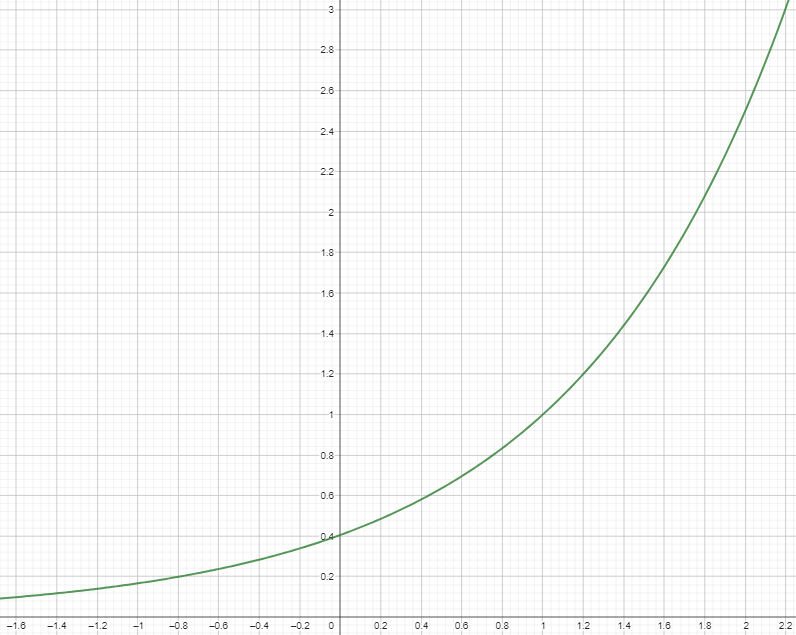
\includegraphics[width=1\textwidth]{../img/img_Lista2/ej3.png}
\end{figure}
\end{enumerate}
\[
\therefore \lim_{x \to 0}\frac{3^x-2^x}{x} \approx 0.405
\]
%2
\section{Ejercicio 9}
\[
\lim_{x \to +\infty}\frac{(2x-1)^5}{(3x^2+2x-7)(x^3-9x)}
\]
Para resolver este límite primero reescribiremos la expresión algebraica.
\[
\frac{(2x-1)^5}{(3x^2+2x-7)(x^3-9x)} = \frac{32x^{5}-80x^{4}+80x^{3}-40x^{2}+10x-1}{3x^{5}+2x^{4}-34x^{3}-18x^{2}+63x} \cdot \frac{\frac{1}{x^{5}}}{\frac{1}{x^{5}}}
\]
\[
\frac{ \frac{32x^{5}-80x^{4}+80x^{3}-40x^{2}+10x-1 }{x^{5}}}{ \frac{3x^{5}+2x^{4}-34x^{3}-18x^{2}+63x}{x^{5}}} = \frac{  \frac{32x^{5}}{x^{5}} - \frac{80x^{4}}{x^{5}} + \frac{80x^{3}}{x^{5}} - \frac{40x^{2}}{x^{5}} + \frac{10x}{x^{5}}- \frac{1}{x^{5}} }{
\frac{3x^{5}}{x^{5}} + \frac{2x^{4}}{x^{5}} - \frac{34x^{3}}{x^{5}} - \frac{18x^{2}}{x^{5}} + \frac{63x}{x^{5}}}
\]
Ahora será más fácil calcular el límite de la función, considarando que un número divido entre un número muy grande tiende a 0.
\[
\lim_{x \to +\infty} \frac{  \frac{32x^{5}}{x^{5}} - \frac{80x^{4}}{x^{5}} + \frac{80x^{3}}{x^{5}} - \frac{40x^{2}}{x^{5}} + \frac{10x}{x^{5}}- \frac{1}{x^{5}} }{
\frac{3x^{5}}{x^{5}} + \frac{2x^{4}}{x^{5}} - \frac{34x^{3}}{x^{5}} - \frac{18x^{2}}{x^{5}} + \frac{63x}{x^{5}}} = \lim_{x \to +\infty}  \frac{  \frac{32x^{5}}{x^{5}} - 0 + 0 - 0 + 0- 0 }{
\frac{3x^{5}}{x^{5}} + 0- 0-0+ 0}
\]
\[
 = \lim_{x \to +\infty}  \frac{\frac{32x^{5}}{x^{5}}}{\frac{3x^{5}}{x^{5}}} = \lim_{x \to +\infty} \frac{32}{3} = \frac{32}{3}
\]
\[
\therefore \lim_{x \to +\infty}\frac{(2x-1)^5}{(3x^2+2x-7)(x^3-9x)} = \frac{32}{3}
\]
%3
\section{Ejercicio 18}
\[
\lim_{\theta \to 0^+} \ln (\sin 2\theta) - \ln (\tan \theta)
\]
Primero reescribiremos la expresión
\[
 \ln (\sin 2\theta) - \ln (\tan \theta) = \ln ( \frac{\sin 2\theta}{\tan \theta} ) 
\]
Considerando la fórmula para el seno de la suma de ángulos $ \sin (\alpha + \beta) = \sin \alpha \cdot \cos \beta + \cos \alpha \cdot \sin \beta $ donde en este caso $\alpha = \beta = \theta$ se puede calcular que $\sin 2\theta = sin \theta \cdot \cos \theta  + \cos \theta  \cdot \sin \theta   = 2 \cdot \cos \theta  \cdot \sin \theta $ \\
Entonces 
\[
 \frac{\sin 2\theta}{\tan \theta} = \frac{ 2 \cdot \cos \theta  \cdot \sin \theta}{\frac{\sin \theta}{\cos \theta}} = \frac{2 \cdot \cos \theta  \cdot \sin \theta \cdot \cos \theta}{sin \theta} = \frac{2 \cdot \sin \theta}{\sin \theta} \cdot [\cos \theta]^{2} = 2 \cdot [\cos \theta]^{2}
\]
\[
\therefore \ln ( \frac{ \sin 2 \theta }{ \tan \theta} ) = ln ( 2 \cdot [\cos \theta]^{2} )
\]
Ahora será más fácil calcular el límite de esta expresión
\[
\lim_{\theta \to 0^+} \ln (\sin 2\theta) - \ln (\tan \theta) = \lim_{\theta \to 0^+}  ln ( 2 \cdot [\cos \theta]^{2} ) =  ln ( \lim_{\theta \to 0^+} ( 2 \cdot [\cos \theta]^{2} )) 
\]
\[
= ln (  2 \cdot [\cos 0]^{2}) =ln (  2 \cdot 1^{2})  = ln (2) 
\]
\[
\therefore \lim_{\theta \to 0^+} \ln (\sin 2\theta) - \ln (\tan \theta) =  ln (2) 
\]
%4
\section{Ejercicio 20}
\[
\lim_{x \to + \infty} (1+\frac{a}{x})^{bx} ~ ~ ~,~ ~ a,b>0
\]

%5
\section{Ejercicio 31}
Encuentre valores de $x$, si los hay, en los que la función dada no sea continua.
\begin{enumerate}[label=(\alph*)]
\item \[ f(x)=\frac{x}{x^2-1} \]
Sabemos que las funciones $y=x$ y $y=x^2-1$ son funciones polinomiales. De modo que son continuas en todo su dominio (para toda $x$); es decir, son continuas sobre $\mathbb R=(-\infty,\infty)$. Ahora, la función $f(x)=\frac{x}{x^2-1}$ es racional, así que es continua siempre que está definida; es decir, en su dominio que es $\{ x ~|~ (x^2-1) \neq 0 \}$. Si $x^2-1=0$, entonces:
\[
x^2-1=0
\]
\[
x^2=1
\]
\[
x=\sqrt{1}
\]
\[
x_0=1 \text{ , } x_1=-1
\]
$\therefore$ La función $f(x)=\frac{x}{x^2-1}$ no es continua en los valores de $x_0=1 \text{ y } x_1=-1$.

\item \[ f(x)= | x^3-2x^2 | \]
\begin{enumerate}
	\item[1)] La función dada es polinomial, por lo que está definida para toda $x$.
	\item[2)] Calculando los límites laterales cuando $x$ se acerca a un punto $a$.
	\begin{itemize}
		\item Límite derecho en $a$:
		\[ 
		\lim_{x \to a^+}f(x) = \lim_{x \to a^+}| x^3-2x^2 | =\lim_{x \to a^+}| a^3-2a^2 |
		\]
		\item Límite izquierdo en $a$:
		\[ 
		\lim_{x \to a^-}f(x) = \lim_{x \to a^-}| x^3-2x^2 | =\lim_{x \to a^-}| a^3-2a^2 |
		\]
	\end{itemize}
	Dado que los límites son iguales, entonces el límite existe para cualquier $a$.
	\item[3)] Por el punto anterior, el valor del límite cuando $x$ tiende a $a$ es igual al valor de la función en $a$.
\end{enumerate}
$\therefore$ La función $f(x)= |x^3-2x^2 |$ es continua para toda $x$.

\item \[ f(x)=\frac{x+3}{~|x^2+3x|~} \]
\end{enumerate}

%6
\section{Ejercicio 36}
Supongamos que $f$ es continua en el intervalo $[0, 1]$, que $f(0) = 2$ y que $f$ no tiene ceros en el intervalo. Demuestre que $f(x) > 0$ para todo $x$ en $[0, 1]$.\\ \\

Podemos utilizar el El Teorema del Valor Intermedio para demostrarlo. Este Teorema enuncia para este caso que, sea N un valor entre f(0) y f (1), cumple que $f(0)<N<f(1)$ ó $f(1)<N<f(0)$ y existe un $c \in (0, 1)$ tal que $f(c) = N$.\\
Lo que queremos demostrar es que $N>0$ para cualquier $c \in (0, 1)$. \\
Considerando que $f(0) = 2 $ podemos considerar que $2<N<f(1)$ ó $f(1)<N<2$  \\
En el primer caso donde la función es creciente, $2<N$ asegura que $N>0$ \\
En el segundo caso, tenemos que considerar que $f(1)>0$ ya que de lo contrario, según el teorema del valor intermedio $f(c)$ tendría que ser $0$ para alguna $c \in (0, 1)$ ya que 0 es un valor intermedio entre $f(0) = 2$ y cualquier número negativo. Ya que se garantiza que no hay ceros en el intervalo [0,1], $f(1)$ debe ser positivo, y por tanto en la desigualdad  $f(1)<N<f(0)$ si $f(1)<N$, entonces N es número positivo y por tanto $N>0$

\end{document}